\clearpage
\article{Хрюникс}{Библиотека \sdl}{

Библиотека \sdl\ (Simple DirectMedia Layer)\ --- свободная
кросс-плат\-фор\-мен\-ная библиотека, созданная для обеспечения низкоуровневого
HAL. Разработчики ПО могут использовать ее для написания компьютерных игр и
других мультимедиа-приложений для множества операционных систем, таких как
Android, iOS, Linux, Mac OS X, Windows\ldots Изначально \sdl\
создавалсь для написания игр, эмуляторов платформ и полноэкранных графических
приложений в старом DOSовском стиле.

\begin{framed}

\fbox{HAL: Hardware Abstraction Layer}

Слой аппаратных абстракций\ --- слой абстрагирования, реализованный в
программном обеспечении, находящийся между физическим уровнем аппаратного
обеспечения и программным обеспечением, запускаемом на компьютере.
HAL предназначен для сокрытия различий в аппаратном обеспечении от основной
части ядра операционной системы и другого низкоурвневого ПО, таким образом чтобы
большая часть кода не нуждалась в изменении при сборке на системах с различным
аппаратным обеспечением.
\end{framed}

\begin{multicols}{2}
\noindent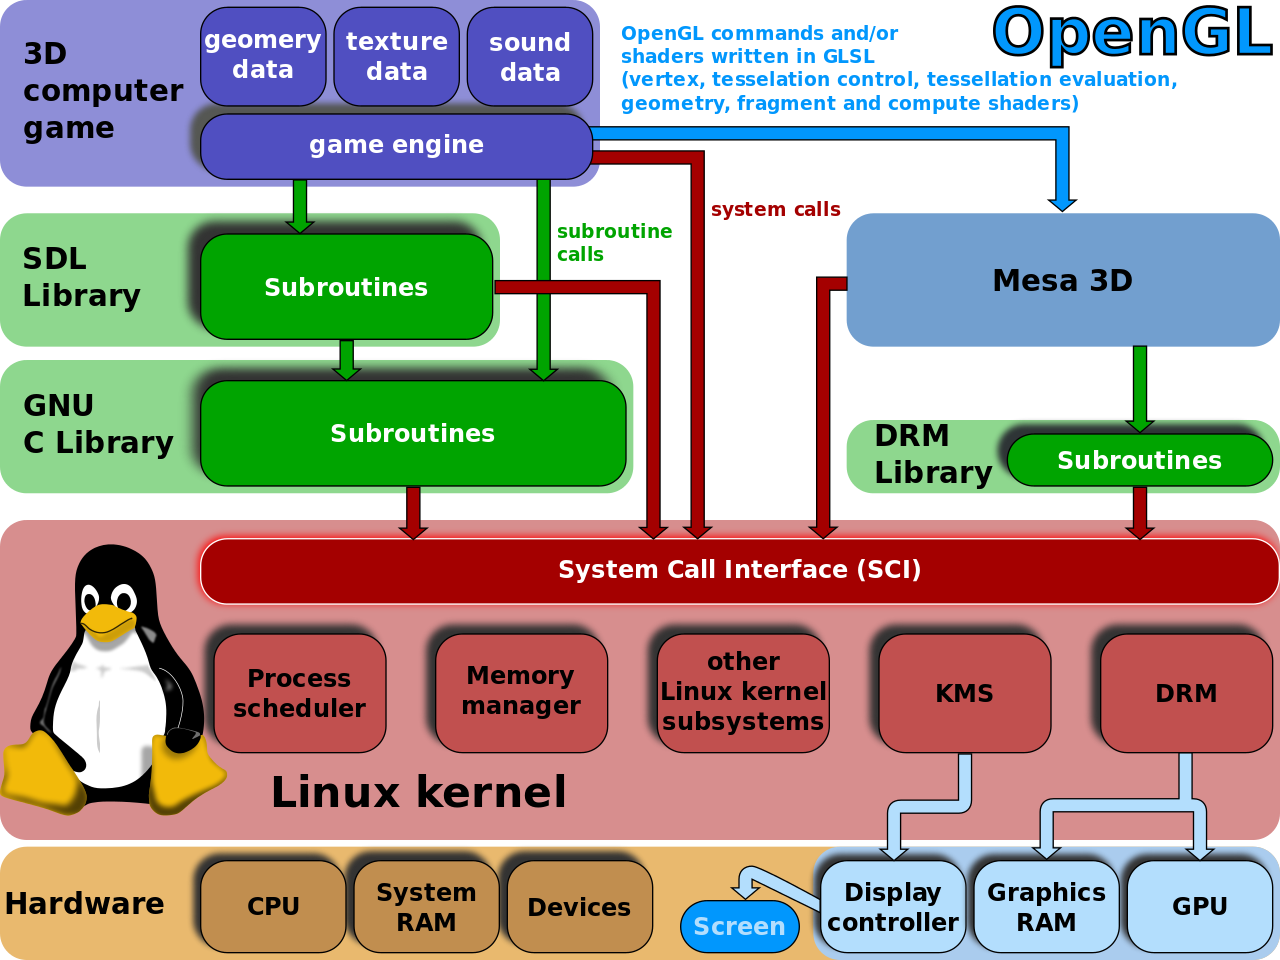
\includegraphics[width=\columnwidth]{01/SDLsheme1.png}
\columnbreak
\noindent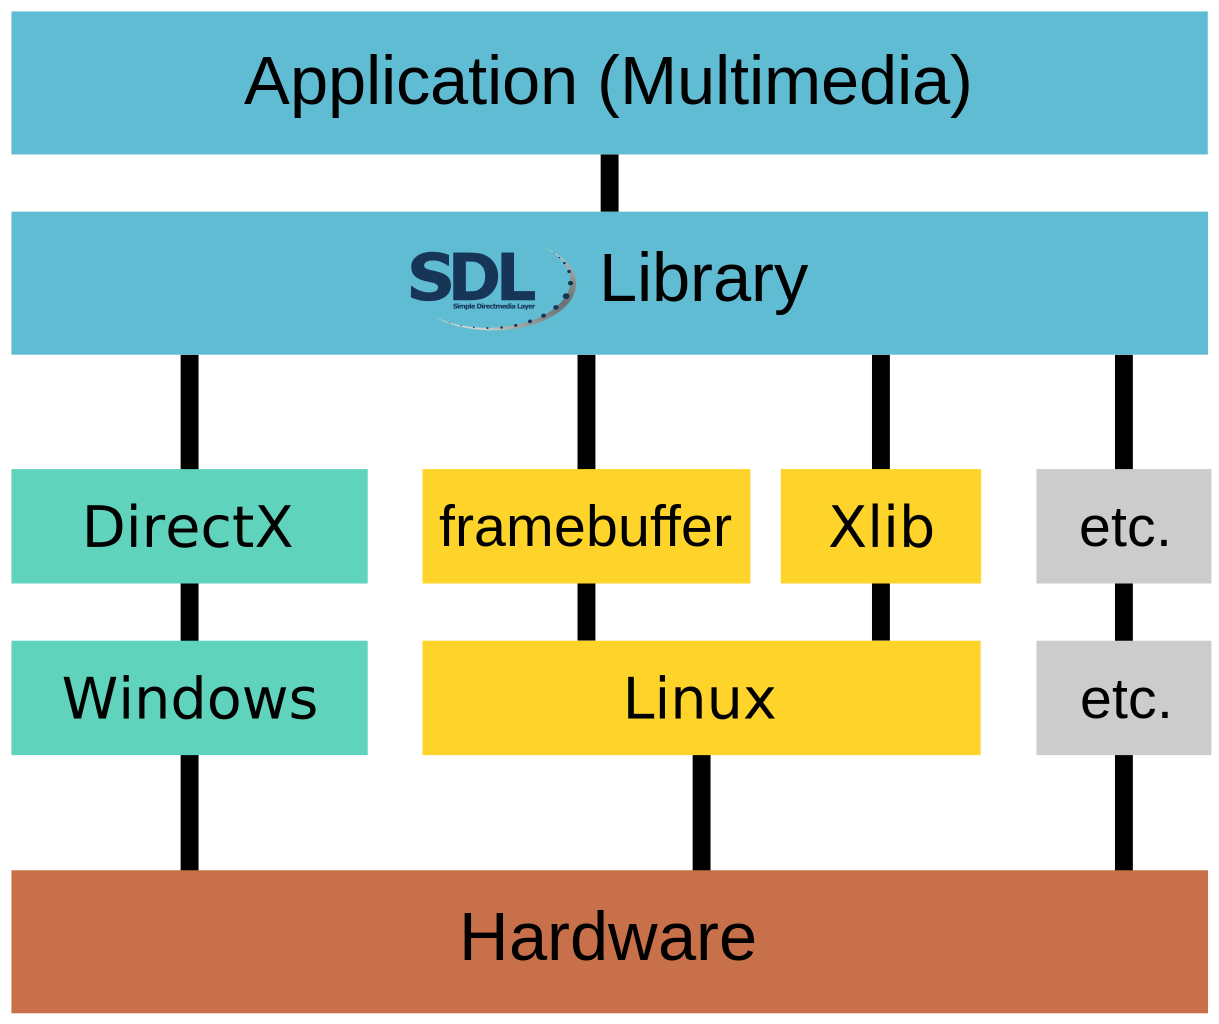
\includegraphics[width=\columnwidth]{01/SDLsheme2.png}
\end{multicols}

\sdl\ поддерживает видео, аудио, усрйства ввода, упрвление CD-ROM, нити,
загрузку разделяемых объектов, сеть и таймеры. Для 3D-графики поддерживется
контекст OpenGL и Direct3D.

Библиотека написана на Си, и также предоставляет прграммный интерфейс на Си, в
тм числе в виде расширений для других языков программирвания.
Она свободна и поставляется в исходных кодах под условиями GNU LGPL (версия 1) и
Лицензией zlib (версия 2). Так как zlib SDL2 свободно доступна для статической
линковки с коммерчестким ПО, она широко используется в больших и маленьких
продуктах. Свыше 700 игр, 180 приложений, и 120 дем также предоставляются с
сайта библиотеки.

Часто упоминается что \sdl\ это игровой движок, но это не так. Тем не менее
библиотека удобна для построения такого движка в кажестве нижнего слоя.

Основная часть \sdl\ содержит базовый, весьма ограниченный спектр возможностей.
Дополнительную функциональность обеспечивают библиотеки расширений, которые
обычно входят в поставку.

\subarticle{Сборка для \emlinux}

Для Cross \linux\ необходимость сборки библиотеки задается в
\make-пе\-ре\-мен\-ной \file{LIBS}: в мейкфайле приложения, \file{user.mk}\ и
\file{.mk}\ отдельных пакетов в эту переменную прописывается список необходимых
библиотек. Затем при сборке мета-пакета \file{libs}\ (\file{user.mk})
выполняется цикл сборки всех библиотек.

Файл сборки \sdl\ включает как основную часть, так и библиотеки-рас\-ши\-ре\-ния
\file{SDL\_*}. Для \file{SDL\_ttf}\ (позволяет использовать в программах
True\-Type/Free\-Type шрифты) также необходима уже собранная библиотека
\file{freetype}.

\lst{config/mk/lib/sdl.mk}{https://github.com/ponyatov/cross/raw/master/config/mk/lib/sdl.mk}{../cross/config/mk/lib/sdl.mk}

\lst{config/mk/lib/freetype.mk}{https://github.com/ponyatov/cross/raw/master/config/mk/lib/freetype.mk}{../cross/config/mk/lib/freetype.mk}

\subarticle{\file{sdlrect}: вывод случайных прямоугольников}

Успешность сборки библиотеки можно проверить, загрузив собранный Cross
\linux\ и ввести команду \file{sdlrect}: будут выводиться случайные цветные
прямоугольники. По скорости их вывода можно визуально оценить скорость работы
эмулятора или железа, если вы запустили сборку на реальном компьютере.

Не забудьте указать в конфиге загрузчика параметр ядра \file{vga=ask}\ или
\file{vga=0x315}\footnote{\ нужный код видеорежима можно узнать запуская с
\file{vga=ask}}. Если ядро не запускается в графическом режиме
\emph{FrameBuffer}, скорее всего вы ошиблись с опциями ядра при его сборке.

Если все нормально, при старте ядра в левом верхнем углу экрана будет выводится
черно-белый логотип \linux. При желании можете его поменять на цветной в файле
\href{https://github.com/ponyatov/cross/raw/master/config/arch/i386/VGA.kernel}{\file{config/arch/i386/VGA.kernel}}.

\lst{user/sdlrect.c}{https://github.com/ponyatov/cross/raw/master/user/sdlrect.c}{../cross/user/sdlrect.c}

\subarticle{\file{sdlclock}: \linux-часы}

А вот теперь настал момент, ради которого все и затевалось\ --- собираем
\file{sdlclock}: приложение электронных линукс-часов. Пока самый простейший
вариант без будильника и плюшек, просто фоновая картинка и дата/время:

\lst{user/sdlclock.c}{https://github.com/ponyatov/cross/raw/master/user/sdlclock.c}{../cross/user/sdlclock.c}

Вы можете заметить секции кода, помещенные макросом \file{WIN32}: компилируя
программу под Windows\MinGW командой \file{gcc -DWIN32 \ldots}\ вы можете быстро
ее отладить, не заморачиваясь со сборкой em\linux. Естественно в MinGW должна
быть установлена соответствующая бинарная сборка \sdl\ для win32, ее можно
скачать с сайта библиотеки.

}{}
